\chapter{Background} \label{chap:back}

As a social species, communication has a keystone role within our species' success, where speech is the most important of many tools that we use to express both thoughts and feelings. Speaking is, for the most part, such an effortless endeavour that we are not aware of both the complex cognitive and precise mechanical processes that are involved. As such, a review of both the functioning of the human vocal apparatus and the speech production mechanism is crucial for introducing the problem at hand. Although for the purpose of this thesis we are mostly concerned with the processing and modeling of speech signals, it is important to understand not only the underlying mechanisms of speech production, as they are the basis for the models and algorithms that are used for speech analysis and synthesis, but also the role of speech within human behavior.

It is relevant to first point out that the role of speech in human interaction is not only to convey information, but also to express emotions, attitudes and intentions. The ability to communicate has allowed human beings to cooperate and form societies, and it is the basis for the development of culture and technology. Paradoxically, despite speech being a tool for cooperation, it is also a tool for conflict, as it can be used to deceive, manipulate and even to incite violence. Some have hypothesized a dominant-subordinate relationship that is present in speech, through the embedding of power dynamics and symbolic violence within not only social structures, but also language itself. This is a topic that has been explored by Žižek \cite{žižek2009violence}, who argues that the belief that language is what makes us human is a myth, and that language is also a tool for violence, especially when it is used to exclude, marginalize or oppress others through means of symbolic violence.

Despite such a complex and multifaceted nature, speech is a very natural yet complex process that involves the production and perception of vocal signals, where the speaker must encode the message in such a way that the listener can decode it. This process involves the use of both the vocal apparatus, which is a complex system responsible for the speech production, and the auditory system, which is responsible for the speech perception. The study of speech production and perception is then a multidisciplinary field that involves the study of human physiology, psychology, linguistics, acoustics, and signal processing, among others.

\section{The human vocal apparatus}

%%
The human vocal apparatus is a very complex system that is responsible for allowing speech production. Thus, its study should be the starting point in any discussion concerning speech coding or conversion as it allows to identify the main signal processing steps involved in the production of both voiced and unvoiced speech, as well as to identify the characteristics and behavior of source signals and filter configurations in both cases. 

Depicted in Figure \ref{fig:vocalApparatus}, the apparatus can be thought as 3 distinct subsystems, the subglottal region, which is composed by the lungs and the trachea, the larynx, which is composed by both the vocal folds and the glottis, and the supraglottal region, which includes the pharynx, the mouth and the nasal cavities

%% TODO: use stealth to caption direction
\begin{figure}[H]
    \centering
    \begin{tikzpicture}[scale=0.8]
        %\pgflowlevelsynccm
        \node[anchor = west] at (0,0) {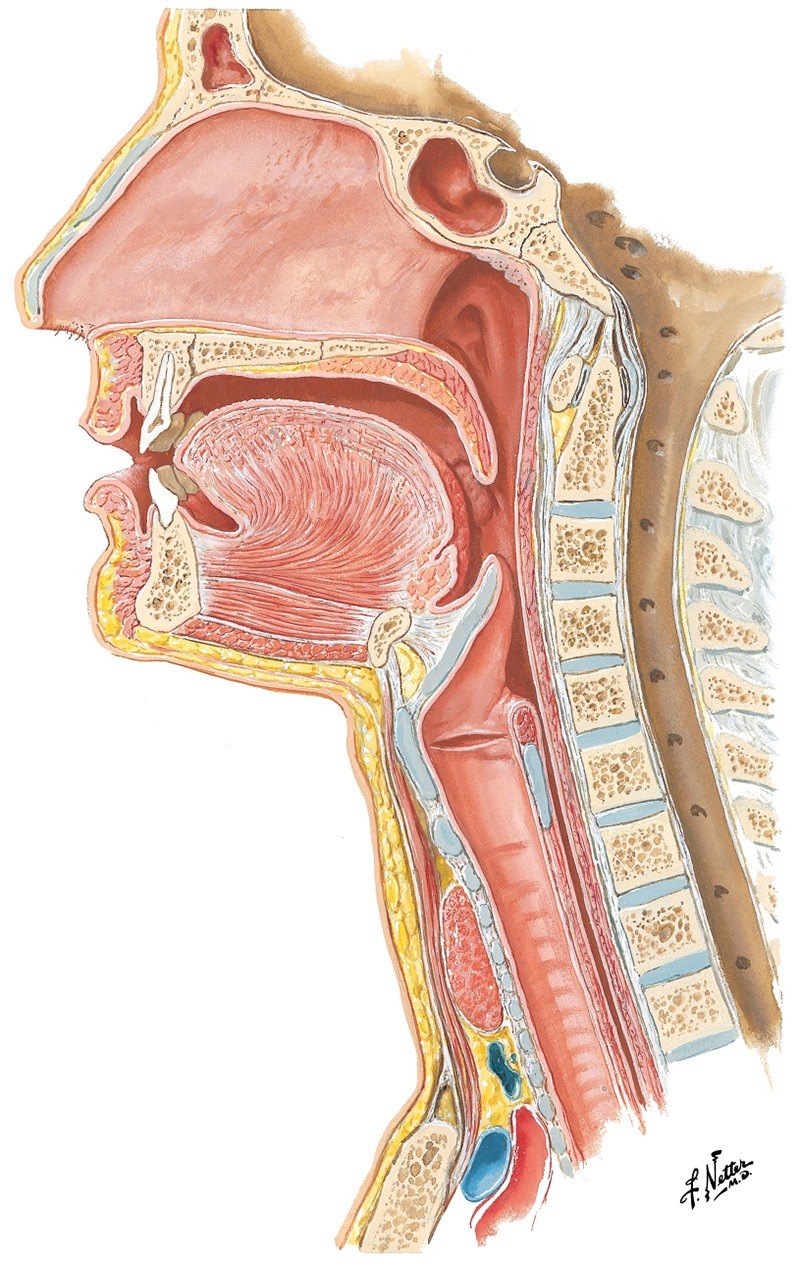
\includegraphics[width=6.4cm]{chapter2/netterVocalApparatus.jpg}};
        %\draw (0, 0) -- (8, 0);
        \draw (6.3, 5.8)--(3.4, 4.31);
        \node[align = center] at (7.5,5.8){nasal cavity};
        \draw (8.5,0)--(4.9, 0.27);
        \node[align = center] at (9.5,0){epiglottis};
        \draw (8.5,2)--(4.9, 2);
        \node[align = center] at (9.1,2){uvula};
        \draw (8.5,-2)--(4.8, -1.15);
        \node[align = center] at (9.5,-2){vocal fold};
        \draw (3.35,-2)--(5.25, -2);
        \node[align = center] at (2.6,-2){trachea};
        \draw (1, 5.8)--(2.8, 2.45);
        \node[align = center] at (0.5, 6){oral cavity};
        \draw (1.1,-1)--(3, 1.5);
        \node[align = center] at (1,-1.25){tongue};
        \draw (0.2, 0.2)--(1.8, 1.3);
        \node[align = center] at (0, 0){teeth};
        \draw (0.3, 2)--(1.2, 2.1);
        \node[align = center] at (0, 2){lip};
    \end{tikzpicture}
    \caption{Human vocal apparatus - adapted from \cite{netterAtlasHumanAnatomy2019}}
    \label{fig:vocalApparatus}
\end{figure}


\subsection{Subglottal Region}

The respiratory system, otherwise referred to as the subglottal region, comprises the lungs, diaphragm and the various airways that facilitate breathing. This system plays a crucial role with speech production by generating the airflow necessary for the vocal apparatus to produce sound. The airflow dynamics within the subglottal region are governed by both the anatomical structure of the respiratory tract and the physiological control mechanisms of breathing.

The lungs are the main part of this system, they're a pair of air-filled organs at each side of the thorax responsible for air exchange. Serving as a reservoir for air, their ability to expand and contract due to the elasticity of the lung tissue enables both the inhalation and exhalation processes. As one speaks, the controlled release of air from the lungs provides the energy source for speech, either exciting the vocal folds into vibration or just exciting the vocal tract (VT). The diaphragm, meanwhile, is a muscle located right below the lungs which contracts while inhaling, creating a vacuum that pulls air into the lungs. A similar function is also performed by the intercostal muscles which are located in between the ribs, by either expanding or contracting the rib cage \cite{zhangMechanicsHumanVoice2016}. 

\subsection{Larynx}

The larynx, often referred to as the voice box, is a crucial component of the phonatory system located in the neck atop the trachea. It is a keystone component of the apparatus, as it directs air towards the vocal folds housed within it, acting as a valve for modulating the airflow and the sound production. The larynx has a complex structure composed of connective tissues, cartilages and muscles which manipulate said cartilages, which allow for precise control over several aspects of the vocal folds such as their position, tension and length of the vocal folds. These, in turn are responsible for modulating the pitch, volume and quality of the speech.

Central to the larynx are two bands of muscle and connective tissue that stretch horizontally across the larynx, these are the vocal folds. The vocal folds are responsible for the production of voiced speech, as they vibrate when air is expelled from the lungs, creating a sound source that is then shaped by the vocal tract. The vocal folds are also responsible for the production of unvoiced speech, as they can be relaxed to allow air to pass through the larynx without any vibration. The glottis, meanwhile, is the space between the vocal folds, and it is responsible for the modulation of the airflow through the larynx.

\begin{figure}[H]
    \centering
    \begin{minipage}[H]{0.495\textwidth}
        \centering
        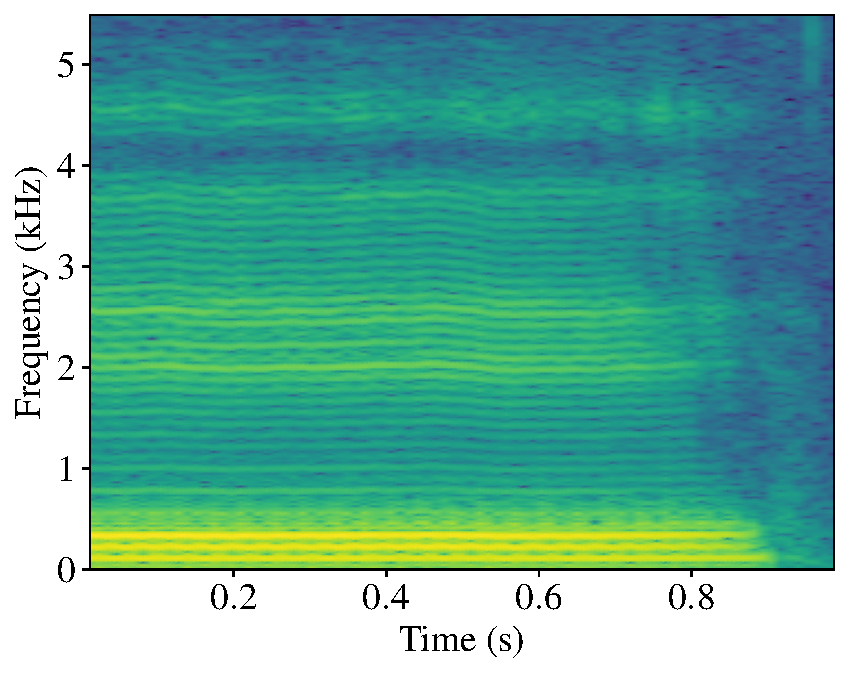
\includegraphics[width=\textwidth]{chapter2/voicedSpectrogram.pdf}
        \subcaption{}
    \end{minipage}
    \begin{minipage}[H]{0.495\textwidth}
        \centering
        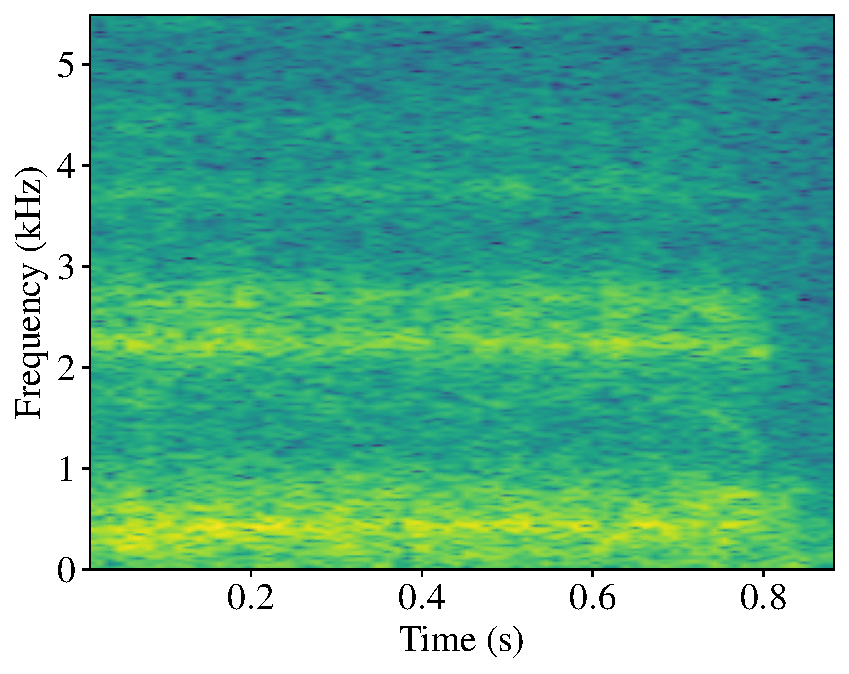
\includegraphics[width=\textwidth]{chapter2/whisperedSpectrogram.pdf}
        \subcaption{}
    \end{minipage}
    
    \caption{\centering Spectral differences between a voiced (left) and unvoiced (right) sustained vowel}
    \label{fig:voicedVsUnvoiced}
\end{figure}

Voiced speech is characterized by the presence of a fundamental frequency, which is the lowest frequency of the harmonic series produced by the vocal folds. This fundamental frequency is then responsible for the pitch of the speech signal, and it is the main difference between voiced and unvoiced speech. Unvoiced speech, on the other hand, is characterized by the lack of a fundamental frequency, as the vocal folds are relaxed and air is expelled through the open glottis. This way, the vocal tract shapes the sound spectrum in a way that the formants are still present, such that vowels are still identifiable, but without any discernable fundamental frequency, nor harmonic structure. Even so, it has been shown that whispered speech has a flatter power spectral density, this results in a noise-like sound that is then shaped by the vocal tract, as can be seen in Figure \ref{fig:voicedVsUnvoiced}.

\subsection{Supraglottal region}

The supraglottal region, encompassing the pharynx, oral cavity, and nasal cavities, forms the vocal tract, which plays a crucial role in shaping the sound produced by the vocal folds. This region acts as a resonating chamber, filtering and coloring the sound to create distinct timbre and articulation in speech. The pharynx, a muscular tube connecting the nasal and oral cavities to the larynx and esophagus, serves as a resonating cavity that amplifies and modifies sound \cite{sundbergFormantStructureArticulation2009}. The position and shape of the pharynx affects the resonant frequencies and quality of the sound produced.

Each of these structures contributes to the articulation and modulation of speech sounds. The lips alter sound by opening or closing, rounding or spreading, essential for producing various vowel and consonant sounds. The teeth provide points of contact for certain consonants, while the tongue, the most flexible articulator, shapes a wide range of speech sounds by touching or approaching different parts of the mouth. The hard palate serves as a surface for the tongue to press against, and the soft palate directs airflow through the oral or nasal cavity, crucial for producing nasal sounds \cite{mcloughlinSpeechAudioProcessing2016}.
 
The nasal cavities, air-filled spaces behind the nose, add unique resonance to the voice, especially for nasalized sounds. Airflow through the nasal cavities, controlled by the soft palate, creates nasal sounds, and the shape and size of these cavities contribute to the voice's overall resonance and quality. The supraglottal region functions as an acoustic filter, shaping the harmonic content of the sound from the vocal folds. This filtering process defines the resonant frequencies, or formants as shown later on, crucial for vowel sounds and speech intelligibility. Formants are influenced by the vocal tract's shape and length, altered by the movement of the tongue, lips, and other articulators \cite{sundbergFormantStructureArticulation2009}.


\section{Speech Modelling}

Having discussed the human vocal apparatus and its role in speech production, it is now important to discuss the models that are used to represent the speech signal, and the digital signal processing techniques that are used for speech analysis and synthesis.

\subsection{Source-Filter model}

%%
The source-filter model describes the human vocal system as a combination of sound sources and filters, relating the articulation of the speech sounds with the features of acoustic signals \cite{ferreiraComunicacoesAudiovisuaisTecnologias2009}. The original model proposed by Fant \cite{Fant1960AcousticTO} relies on the simplifying assumption that source and the filter are independent, i.e. it ignores coupling effects between these.

As per this model, there are two types of sound sources, a periodic and a non periodic one, representing the vocal folds vibration and turbulent air excitation, respectively. The filters represent the supraglottal system, namely the vocal tract, whose resonances represent the filter formants, and the radiation characteristics. A overview of this model can be seen in Figure \ref{fig:sourceFilterModel}.

\begin{figure}[H]

    \centering
    \begin{tikzpicture}
        % Outer box
        \draw (-4, -3) rectangle ++(5, 6);

        % Nodes
        \node (sum2) [draw, circle] {+};
        \node (pulse) [draw, rectangle, above left=of sum2, minimum width = 2cm, minimum height = 1cm] {Pulses};
        \node (noise) [draw, rectangle, below left=of sum2, minimum width = 2cm, minimum height = 1cm] {Noise};
        \node (vocalTract) [draw, rectangle, right= 2cm of sum2, align=center, minimum width = 2.5cm, minimum height = 1.5cm] {Vocal Tract \\ Filter $H(z)$};
        \node (lipRadiation) [draw, rectangle, right= 2cm of vocalTract, align=center, minimum width = 2.5cm, minimum height = 1.5cm] {Lip Radiation \\ Filter $L(z)$};

        % waveforms
        \node at (-0.25, 2.4) {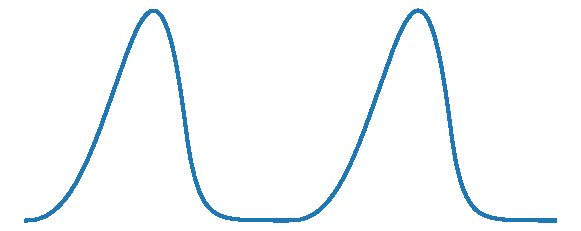
\includegraphics[width=1.5cm]{chapter2/sourceFilterDiagram/lfWave.pdf}};
        \node at (-0.25, -2.4) {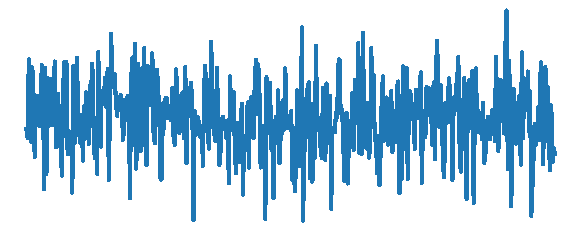
\includegraphics[width=1.5cm]{chapter2/sourceFilterDiagram/noise.pdf}};
        \node at (1.2, 0.3) {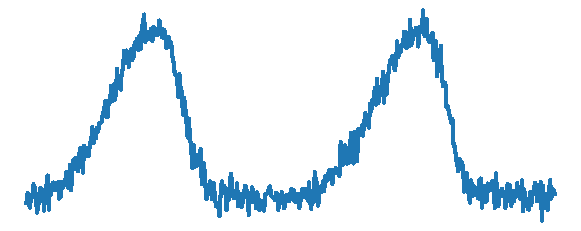
\includegraphics[width=1.5cm]{chapter2/sourceFilterDiagram/pulseNoise.pdf}};
        \node at (5.8, 0.3) {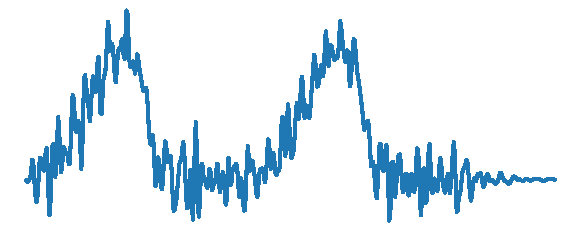
\includegraphics[width=1.5cm]{chapter2/sourceFilterDiagram/ZEROfiltered.pdf}};
        \node at (10.2, 0.3) {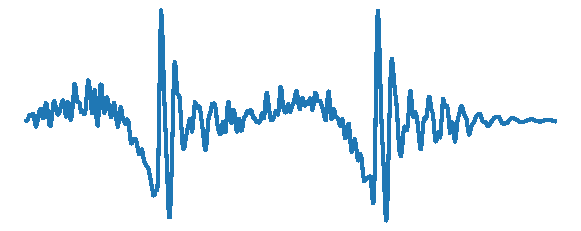
\includegraphics[width=1.5cm]{chapter2/sourceFilterDiagram/filtered.pdf}};
 
        % source/output circles
        \draw (pulse.east) ++(0.6cm, 0) circle (1mm);
        \draw (noise.east) ++(0.6cm, 0) circle (1mm);
        \draw (lipRadiation.east) ++(1.5cm, 0) circle (1mm);

        % Arrows
        \draw (pulse.east) -- ++(5mm, 0);
        \draw (noise.east) -- ++(5mm, 0);
        \draw (lipRadiation.east) -- ++(14mm, 0);
        \draw [-stealth] (sum2) -- ++(-0.6cm, 1.62cm);
        \draw [-stealth] (sum2) -- (vocalTract);
        \draw [-stealth] (vocalTract) -- (lipRadiation); 

    \end{tikzpicture}

    \caption{Source Filter Model of Voice Production}
    \label{fig:sourceFilterModel}
\end{figure}

\subsection{Glottal Flow}

Accurate and realistic estimation models of the glottal flow have been one of the most important aspects of speech synthesis and voice research. This is motivated by both the importance of the glottal flow in the speech production process and the need to understand the operational principles of the vocal folds, but also by the need to develop more efficient and realistic systems for speech synthesis or voice conversion. Here, a brief overview of some of the most important models for the glottal flow will be presented.

It is relevant to point out that the glottal flow is a measure of raw airflow through the glottis along time. However in most speech synthesis applications we are mostly concerned with the glottal flow derivative, as labial radiation can be approximated with a first order derivative filter \cite{doval:hal-00368131, Murphy2011DigitalSP}. Another important aspect of the glottal flow is that of spectral tilt, which is the difference in energy between the higher and lower frequencies of the glottal flow, which is an important aspect of voice quality and speech analysis \cite{ferreira2018on}.

%\textit{Devia explicar o spectral tilt aqui também?}


\subsubsection{Liljencrants-Fant model}

The Lijencrants-Fant (L-F) model \cite{fantFourparameterModelGlottal1985} is a five parameter mathematical model that was developed in order to represent the glottal flow during phonation, aiming to capture the physics behind the glottal flow, making it very widely used in speech synthesis and overall voice research. It is described as a piecewise mathematical function, as represented in Equation (\ref{eq:lfDerivative}), where the glottal flow derivative is described with one formula for first the opening phase, and another for the closing phase:

\begin{equation}
    g'_{LF}(t) = 
    \begin{cases}
        E_0 e^{\alpha t} \sin{\omega_g t} & , 0 \le t \le T_e \\
        - \frac{E_e}{\epsilon T_a} (e^{-\epsilon(t-T_0)} - e^{-\epsilon(T_0- T_e)}) & , T_e \le t \le T_c = T_0
    \end{cases}
    \label{eq:lfDerivative}
\end{equation}

One characteristic of the LF model is that its derivative complies with the condition that its integral across one complete period is null, this ensures that the glottal flow is volume-conserved \cite{fantFourparameterModelGlottal1985}. The glottal flow and the glottal source flow can be seen in Figure \ref{fig:lfModelGraph}. The model is defined by the parameters $E_0$ which is the maximum flow, $\alpha$ which is the damping factor, $\omega_g$ which is the angular frequency, $T_e$ which is the opening time, $E_e$ which is the end flow, $\epsilon$ which is the damping factor for the closing phase, $T_a$ which is the closing time, and $T_0$ which is the period of the glottal flow.

\begin{figure}[H]
    \centering

    \begin{minipage}[H]{0.495\textwidth}
        \centering
        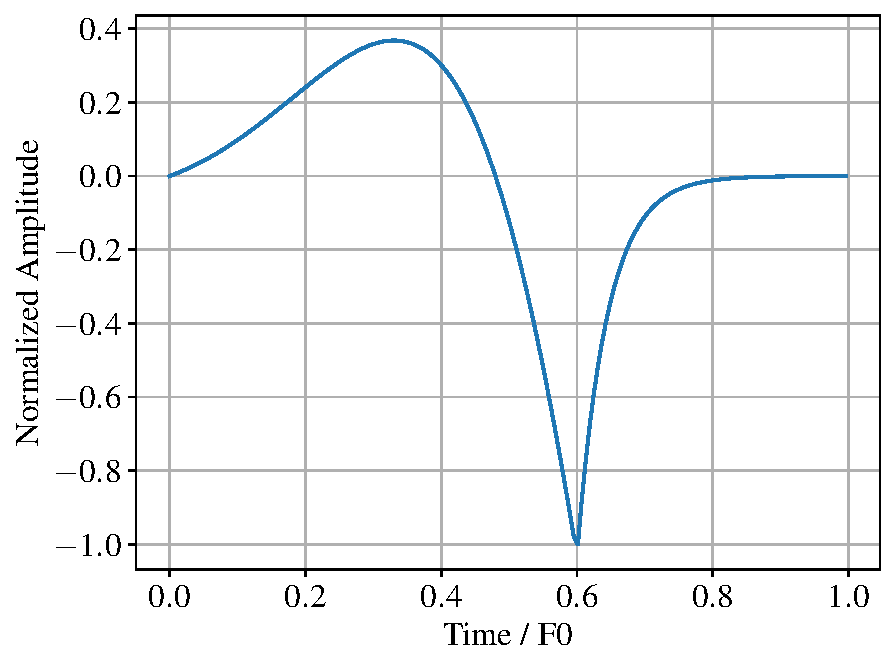
\includegraphics[width=\textwidth]{chapter2/lfFlowDerivative.pdf}
        \subcaption{}
    \end{minipage}
    \begin{minipage}[H]{0.495\textwidth}
        \centering
        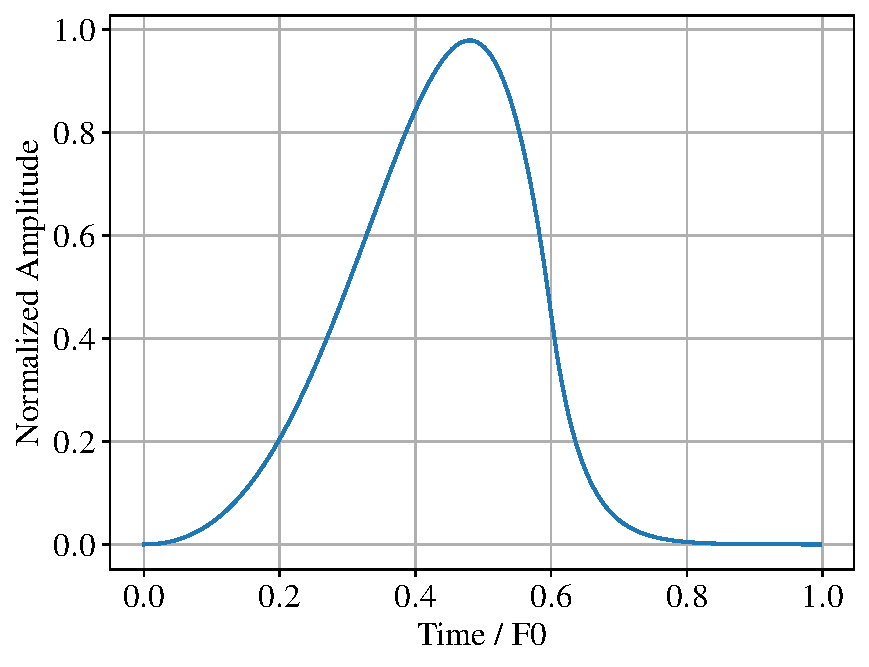
\includegraphics[width=\textwidth]{chapter2/lfFlow.pdf}
        \subcaption{}
    \end{minipage}

    \caption{\centering Lijencrants-Fant glottal flow model derivative (left) and\\corresponding glottal source flow (right)}
    \label{fig:lfModelGraph}
\end{figure}

\subsubsection{Rosenberg model}

Meanwhile, the model proposed by Rosenberg \cite{rosenbergEffectGlottalPulse1971} is a simpler model that is based on the LF model, but with a simpler mathematical representation, here shown in Equation (\ref{eq:rosenbergDerivative}). The model is composed of three parts, the first part is a sine wave that represents the opening phase, the second part is a sine wave that represents the closing phase and the third part is a null function that represents the closed phase. The glottal flow and the glottal source flow can be seen in Figure \ref{fig:rosenbergModelGraph}.

\begin{equation}
    g'_{ros}(t) = 
    \begin{cases}
        \frac{\pi A}{2T_p} \sin{\pi \frac{t}{T_p}} & 0 \le t \le T_p \\
        -\frac{\pi A}{2T_n} \sin{\frac{\pi}{2} \frac{t-T_p}{T_n}} & T_p \le t \le T_p + T_n \\
        0 & T_p + T_n \le t \le T_0
    \end{cases}
    \label{eq:rosenbergDerivative}
\end{equation}

\begin{figure}[H]
    \centering
    \begin{minipage}[H]{0.495\textwidth}
        \centering
        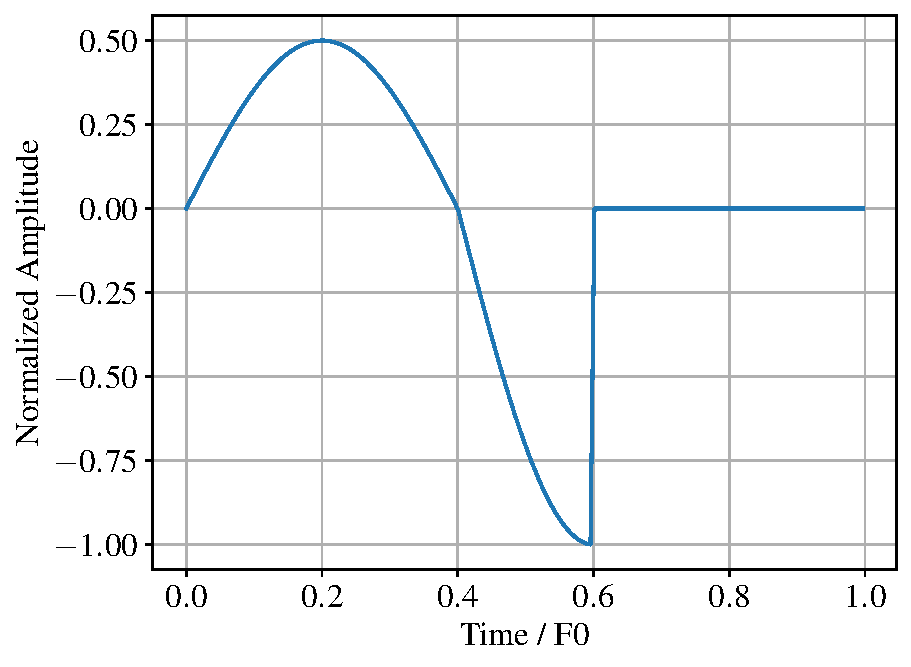
\includegraphics[width=\textwidth]{chapter2/rosenbergFlowDerivative.pdf}
        \subcaption{}
    \end{minipage}
    \begin{minipage}[H]{0.495\textwidth}
        \centering
        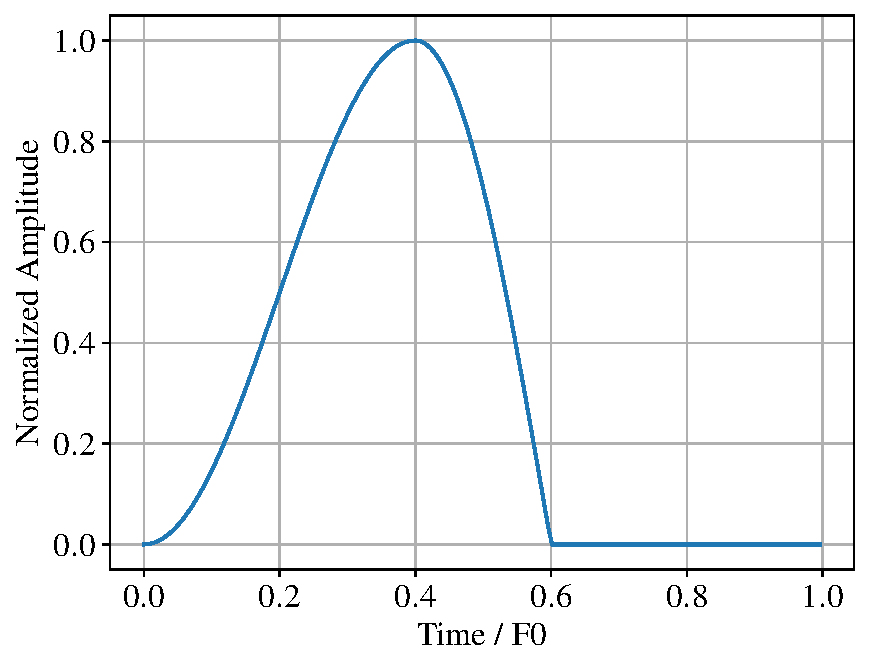
\includegraphics[width=\textwidth]{chapter2/rosenbergFlow.pdf}
        \subcaption{}
    \end{minipage}
    
    \caption{\centering Rosenberg glottal flow model derivative (left) and\\corresponding glottal source flow (right)}
    \label{fig:rosenbergModelGraph}
\end{figure}

\subsubsection{Other Glottal Flow Models}

Both the LF and Rosenberg models presented previously are just two of the many models that have been proposed to represent the glottal flow, and in this case they are both time domain models. These prove quite useful for most applications as the timing of glottal phases such as the opening time and the fundamental period are quite important for modelling the glottal flow \cite{doval:hal-00368131}. Other time domain models of the glottal flow include those proposed by Klatt and Fujisaki et. al \cite{klattAnalysisSynthesisPerception1990, 1169239}.

%Despite this, frequency-domain models are also of interest when concerning speech synthesis and processing. It has been shown that that some of the most relevant parameters for the description of voice quality are described in the frequency domain. 

\subsection{Vocal Tract Filter}

The filtering part of the source-filter model, as depicted in Figure \ref{fig:sourceFilterModel} represents the vocal tract, which is responsible for shaping the sound that is produced by the source part of the model, be it periodic glottal pulses or noisy excitation from the open glottis. This filter thus represents the joint contribution of the pharynx, the oral cavity and the nasal cavity, which are responsible for the resonances of the vocal tract, the formants \cite{doi:10.1044/jshr.3001.122}.

\subsubsection{Formants}

The different resonances and anti-resonances of the vocal tract, which result from the varying vocal tract shapes, define the frequency response of the VT filter and are known as formants. These formants are the peaks in the frequency response of the vocal tract filter, and they are responsible for the timbre of the speech signal, as they define the spectral envelope of the speech signal. 

The first three formants are generally regarded as the most contributive to the correct perception of different vowels, as they are the most prominent in the frequency response of the vocal tract filter \cite{mcloughlinSpeechAudioProcessing2016}. In fact, it is possible to synthesize direct formant frequencies in such a way as to convert a complex speech signal to just as little as 3 harmonics in what is referred to as sinewave speech \cite{Ellis2003_sws}, which can be decoded as actual speech despite sounding completely unintelligible at first. 

\begin{figure}[H]
    \centering
    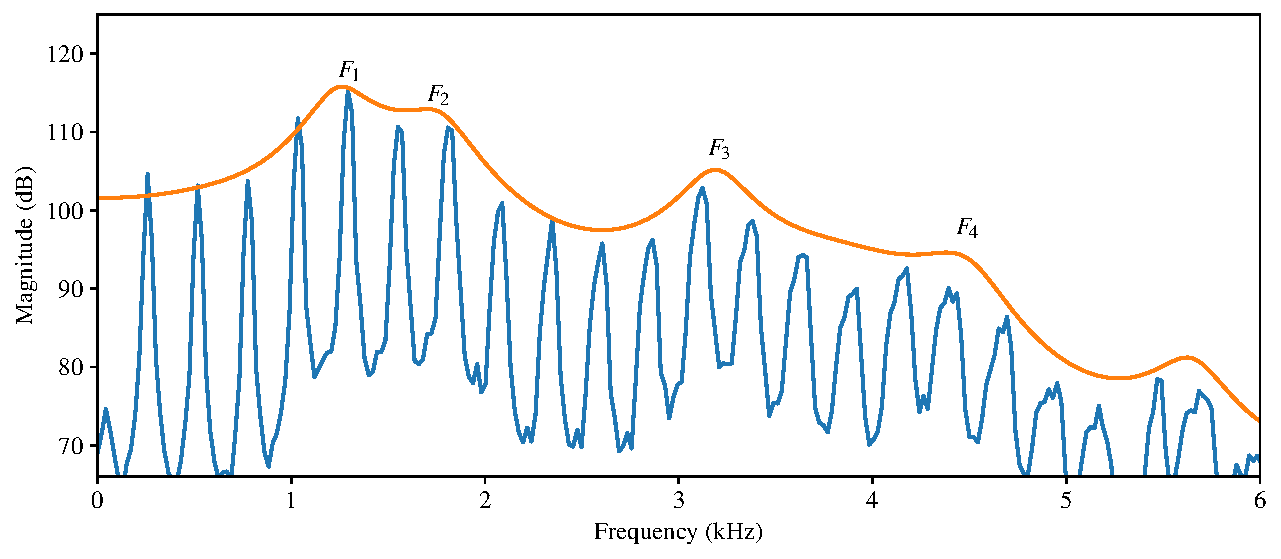
\includegraphics[width=\textwidth]{chapter2/formants.pdf}
    \caption{Formant frequencies, /a/ vowel}
    \label{fig:formants}
\end{figure}

Figure \ref{fig:formants} shows a representation of the spectral envelope (orange) for a given vowel, which was estimated from the original signal spectrum (blue) which has a clear periodic structure due to the period excitation that generated it. The formants are the peaks in the orange spectrum, and they are responsible for the timbre of the speech signal, as they define the spectral envelope of the speech signal. 

\subsubsection{Linear Predictive Coding}

Linear Predictive Coding (LPC) is possibly the most widely used method of estimating the spectral envelop, such as the one shown in Figure \ref{fig:formants}. LPC works through the assumption that an input speech signal can be approximated by a linear combination of its past samples, which is then used to estimate the filter coefficients of the vocal tract filter \cite{hayes1996statistical}. The result of LPC analysis results in a linear all-pole filter, as represented in the z-domain in Equation (\ref{eq:lpcFilter}), that best models the spectral envelope of the speech signal, which can then be used to synthesize speech signals. In fact, LPCs are most widely used in speech coding and synthesis, as they provide a good trade-off between complexity and accuracy \cite{mcloughlinSpeechAudioProcessing2016}. Often the process of estimating the filter coefficients from the spectral envelope is referred to as inverse filtering, as it is the inverse of the process of filtering the source signal with the vocal tract filter.

The process also allows for the spectral envelope of the signal to be removed, thus allowing for the residual signal to be analyzed such that the source signal can be coded into a more compact representation. This is the basis for many speech coding algorithms, such as the Mixed Excitation Linear Prediction (MELP) or Code-Excited Linear Prediction (CELP) algorithms \cite{LinearPredictionCoding2003}.

\begin{equation}
    H(z) = \frac{b_0}{1 - \sum_{i=1}^{p} a_i z^{-i}}
    \label{eq:lpcFilter}
\end{equation}

To calculate the LPC coefficients, several methods can be used but most commonly, the autocorrelation method is utilized in order to compute the $a_k$ filter denominator coefficients. As the name implies, it is based on the autocorrelation sequence $r(n)$ of the input signal $x(n)$, and can be formulated as shown in equation \ref{eq:yulewalker}. This set of equations is known as the Yule-Walker equations, and they can be solved using a least squares method, which is the most common method for estimating the LPC coefficients \cite{jackson1996digital}.

\begin{equation}
    \begin{bmatrix}
        r(0) & r(1)^* & \dots & r(N-1)^* \\
        r(1) & r(0) & \dots & \vdots \\
        \dots & \dots & \ddots & r(2)^* \\
        r(N-1) & r(N-2) & \dots & r(0) \\
    \end{bmatrix}
    \begin{bmatrix}
        a_1 \\
        a_2 \\
        \vdots \\
        a_N
    \end{bmatrix}
    =
    \begin{bmatrix}
        -r(2) \\
        -r(3) \\
        \vdots \\
        -r(N)
    \end{bmatrix}
    \label{eq:yulewalker}
\end{equation}

This being a Toeplitz system of equations, it can be solved efficiently using the Levinson-Durbin recursion \cite{hayes1996statistical}, which is an efficient algorithm that recursively estimates the filter coefficients by minimizing the prediction error. The filter coefficients are estimated by solving the Toeplitz system of equations, which is obtained from the autocorrelation function of the speech signal. In chapter \ref{chap:filt}, the implementation details of this algorithm and the computation of the autocorrelation coefficients are both discussed.

%\section{Phonetics}


